\documentclass{beamer}
\usepackage[utf8]{inputenc}
\usepackage{graphicx}
\usetheme{default}
\usecolortheme{default}

\title[S01 Intro]{Section 01 : Introduction du cours}
\subtitle{GSF-3100 Marché des capitaux}
\author[SP. Boucher]{Simon-Pierre Boucher\inst{1}}
\institute[Université Laval]
{
  \inst{1}%
  Département de finance, assurance et immobilier\\
  Faculté des sciences de l'administration\\
  Université Laval}
\date[Automne 2021]{1 Septembre 2021}

\begin{document}

\begin{frame}
  \titlepage
\end{frame}


\begin{frame}{Table des matières}
\tableofcontents
\end{frame}


\section{Matériel didactique}
\begin{frame}{Matériel didactique}{Introduction}
  \begin{block}{Bond markets, analysis and strategies (9e édition)}
\begin{itemize}
\item Ce livre est recommandé, mais non obligatoire.
\item Auteur(s) : Fabozzi, Frank J.
\end{itemize}
\end{block}
\begin{center}
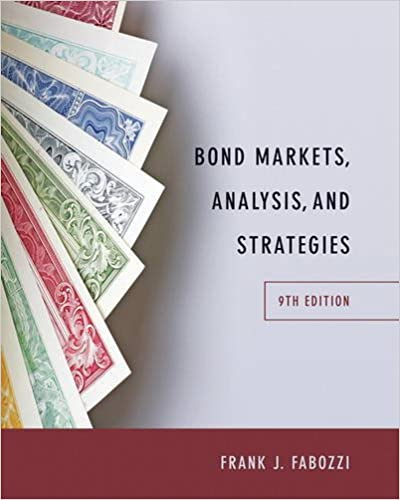
\includegraphics[scale=0.25]{BOOK}
\end{center}
\end{frame}

\section{Évaluations sommatives}
\begin{frame}{Évaluations sommatives}{Introduction}
  \begin{block}{Examen intra}
\begin{itemize}
\item Période de disponibilité : 	le 20 oct. 2021 de 18h30 à 21h20
\item Durée : 2 h 50 min
\item Pondération : 40\% de la note finale 
\item Type : Questions à choix multiples (50 questions)
\item Déroulement :  à distance 
\item Matière à l'examen : Section 01 à 08 inclusivement 
\end{itemize}
\end{block}
\end{frame}

\begin{frame}{Évaluations sommatives}{Introduction}
  \begin{block}{Examen final}
\begin{itemize}
\item Période de disponibilité : le 3 déc. 2021 de 18h30 à 21h20
\item Durée : 2 h 50 min
\item Pondération : 40\% de la note finale 
\item Type : Questions à choix multiples (50 questions)
\item Déroulement :  à distance 
\item Matière à l'examen : Section 09 à 10 inclusivement 
\end{itemize}
\end{block}
\end{frame}


\begin{frame}{Évaluations sommatives}{Introduction}
  \begin{block}{Travail de session}
\begin{itemize}
\item Date de remise : 30 nov. 2021 à 23h59
\item Pondération : 20\% de la note finale 
\item Type : Questions à choix multiples (50 questions)
\item Équipe : Quatre ou cinq étudiants
\item Le travail de session consiste à effectuer une étude approfondie de titres du marché des capitaux reliés au cours.
\end{itemize}
\end{block}
\end{frame}


\section{Objectif du cours}
\begin{frame}{GSF-3100: Marché des capitaux}{Introduction}
  \begin{block}{Objectif du cours:}
\begin{itemize}
\item Étudier les marchés financiers, ainsi que les actifs qui leur sont associés, dans leur rôle d’intermédiaire aux transferts de fonds entre les entités économiques déficitaires et les entités économiques excédentaires, et aux transferts de fonds de façon à redistribuer le risque. 
\item  Le cours se concentre sur les actifs reliés aux marchés des titres à revenu fixe ayant une échéance de moyenne ou longue durée.
\end{itemize}
  \end{block}
\end{frame}

\begin{frame}{GSF-3100: Marché des capitaux}{Introduction}
  \begin{block}{Plan de travail en trois parties:}
\begin{itemize}
\item Concepts de base du marché obligataire.
\item Les marchés d'intermédiation de fonds de financement.
\item Les marchés d’intermédiation de fonds de risque.
\end{itemize}
  \end{block}
  
  \begin{block}{Le but de cet introduction est:}
\begin{itemize}
\item De comprendre le concept de marché d’intermédiation.
\item De clarifier la différence entre les marchés de fonds de financement et ceux de fonds de risque.
\item D’introduire le marché obligataire.
\end{itemize}
  \end{block}
\end{frame}

\section{Actif financier}
\begin{frame}{Actif financier}{Introduction}
\begin{itemize}
\item Définition: Promesse ou obligation d’honorer des engagements financiers.
\item Valeur: Valeur présente de ses flux monétaires.
\item  Rôles:
\begin{itemize}
\item Transfert de fonds entre les entités économiques déficitaires et les entités économiques excédentaires.  (\textbf{Fonds de financement.})
\vspace{0.5cm}
\item Transfert de fonds de façon à redistribuer le
risque.  (\textbf{Fonds de risque.})
\end{itemize}
\end{itemize}
\end{frame}

\section{Intermédiation financière}
\begin{frame}{Intermédiation financière}{Introduction}
\begin{block}{Définition:}
Transformation d’actifs financiers sous forme de « nouveaux » actifs ou titres financiers préférables aux yeux des investisseurs.
\end{block}
\begin{block}{Exemples:}
\begin{itemize}
\item \textbf{Banque:} \\ Prêts, hypothèques $\rightarrow$ compte
d’épargne, certificat de dépôt.
\item \textbf{Compagnie d’assurance:} \\ Obligations, hypothèques $\rightarrow$ polices d’assurances
\end{itemize}
\end{block}

\end{frame}

\begin{frame}{Intermédiation financière}{Introduction}
\begin{block}{Types:}
\begin{itemize}
\item \textbf{Intermédiation de financement} (projets, maison, etc.).
\item \textbf{Intermédiation de risque} (liquidité échéance, défaut, taux d’intérêt, diversification, etc.).
\end{itemize}
\end{block}
\begin{block}{Catégories d’intermédiaires financiers:}
\begin{itemize}
\item \textbf{Institutions financières} (ex: banque, compagnie
d’assurance, société de placements, etc.).
\item \textbf{Marchés financiers}.
\end{itemize}
\end{block}

\end{frame}

\section{Marché financier}
\begin{frame}{Marché financier}{Introduction}
\begin{itemize}
\item \textbf{Définition: Intermédiaire (lieu ou mécanisme) où s’échangent des actifs financiers.}
\item \textbf{Rôles secondaires:}
\begin{itemize}
\item Déterminer les prix.
\item Augmenter la liquidité.
\item Réduire les coûts de transaction.
\end{itemize}
\end{itemize}
\end{frame}

\begin{frame}{Marché financier}{Introduction}
\textbf{Classifications importantes:}
\begin{block}{Par type de titres:}
\begin{itemize}
Obligations et actions
\end{itemize}
\end{block}
\begin{block}{Par échéance:}
\begin{itemize}
\item Marché monétaire (terme $<$ 12 mois).
\item Marché des capitaux (terme $>$ 12 mois).
\end{itemize}
\end{block}
\begin{block}{Nouvelle émission ou non:}
\begin{itemize}
Primaire vs.  secondaire
\end{itemize}
\end{block}
\begin{block}{Livraison:}
\begin{itemize}
Au comptant (spot) vs.  À terme.
\end{itemize}
\end{block}
\end{frame}

\section{Titre à revenu fixe}
\begin{frame}{Titre à revenu fixe}
\begin{block}{Définition:}
Instrument de dette qui requière à l’émetteur/emprunteur de repayer à l’investisseur/prêteur le montant emprunté plus les intérêts sur une période de temps spécifié et selon les termes du contrat.
\end{block}
\begin{block}{Acte de fiducie:}
Contrat entre l’émetteur/emprunteur et l’investisseur/prêteur qui spécifie les obligations de l’émetteur/emprunteur.
\end{block}
\end{frame}




\begin{frame}{Titre à revenu fixe}
\begin{block}{Caractéristiques:}
\begin{itemize}
\item Type d’émetteur (gouvernement, firme, etc.).
\item Échéance ou maturité à terme.
\item Valeur nominale (principal) et taux de coupon.
\item Amortissement (cédule de paiement du principal pendant la vie du titre).
\item Provisions (contraintes sur la liquidité, l’endettement, etc.).
\item Garanties (biens immobiliers, maison, etc.).
\item  Clauses optionnelles (rachat, conversion, etc.).
\item CUSIP (code unique identifiant le titre).
\end{itemize}
\end{block}

\end{frame}



\begin{frame}{Titre à revenu fixe}
\begin{block}{Risques}
\begin{itemize}
\item Taux d’intérêt.
\item Réinvestissement.
\item Rachat.
\item Crédit et défaut.
\item Inflation.
\item Taux de change.
\item Liquidité.
\item Volatilité.
\item Autres.
\end{itemize}
\end{block}

\end{frame}


\end{document}
